\icode[magenta]{E-MCH-CA-L4-261025-001}
如图，在倾角为\(\theta\)的山坡平面上有一门大炮，大炮相对于山坡的仰角为\(\alpha\)，发射炮弹的初速为\(v_0\)。试求能达到最大射程的仰角和最大射程，忽略空气阻力。

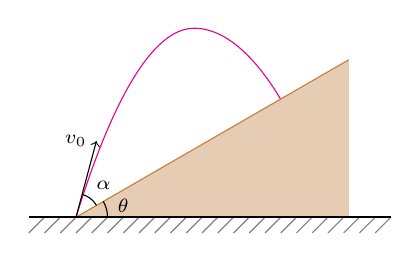
\begin{tikzpicture}[font=\scriptsize]
	\draw[magenta] (0,0) parabola bend(1.5,2.4) (30:3);
	\draw[fill=brown!40,draw=brown] ({4*cos{30}},0)--(0,0)--(30:4);
	\draw (.4,0) arc(0:30:.4);
	\draw (30:.3) arc(30:75:.3);
	\draw[->] (0,0)--(75:1)node[left]{ \(v_0\)};
	\foreach \x in {-.6,-.4,...,4}
		\draw[gray] (\x,-.2)--++(.2,.2);
	\draw[thick] (-.6,0)--(4,0);
	\node at(.6,.15){ \(\theta\)};
	\node at(.35,.4){ \(\alpha\)};
\end{tikzpicture}
